\begin{minipage}{0.45\textwidth}
    \begin{figure}[h]
    \centering
    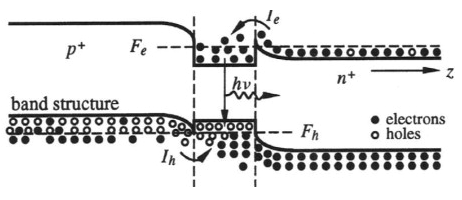
\includegraphics[width=1.1\textwidth]{images/hh-ee.png}
    % \caption{}
    %\label{fig:}
\end{figure}
\end{minipage}
\hfill
\begin{minipage}{0.49\textwidth}
    In the active layer we obtain the Schr\"odinger equation:
    \begin{equation*}
	H_{\text{crystal}} \Psi_n(\vc{r}) = \bigg[\frac{[\vc{p} + e \vc{A}(\vc{r}, t)]^2}{2 m_0}
\end{equation*}
\begin{equation}
	 + U_p(\vc{r})\bigg] \Psi_n(\vc{r})
\end{equation}
\end{minipage}

which will help us to state the induced polarization in an active region:
\begin{equation}
	\mathcal{P}_{in}(\vc{r}, t) = - \sum \frac{\xi(\vc{r},k_q, x, z)}{V(k_q, x, z)}[\rho_{eh}(k_q, x, z)\mu(k_q, x, z) + \const]	
\end{equation}
